\documentclass{beamer}

\usepackage{beamerthemesplit}
\usepackage{amsmath}
\usepackage{amsfonts}
\usepackage{amssymb}
\usepackage{qtree}
\usepackage{cancel}
\usepackage{tkz-graph}
%\usepackage[pdftex]{graphicx}

\mode<presentation>
{
  \usetheme{Warsaw}
  % or ...

  %\setbeamercovered{transparent}
  % or whatever (possibly just delete it)
}


\usepackage[english]{babel}
% or whatever

\usepackage[latin1]{inputenc}
% or whatever

\usepackage{times}
\usepackage[T1]{fontenc}

\title{Program Representation for General Intelligence}

\subtitle{The Reduct Toolkit for Program Normalization}

\author{Nil Geisweiller}

\institute[Xiamen University] % (optional, but mostly needed)
{
  Novamente LLC
}

\date[Xiamen University AGI Summer School 2009] % (optional, should be abbreviation of conference name)
{Xiamen University\\ AGI Summer School 2009}


\AtBeginSection[]
{
  \begin{frame}<beamer>{Outline}
    \tableofcontents[currentsection,currentsection]
  \end{frame}
}

\AtBeginSubsection[]
{
  \begin{frame}<beamer>{Outline}
    \tableofcontents[currentsection,currentsubsection]
  \end{frame}
}

%\newcommand{\AND}{\textit{AND}}
%\newcommand{\OR}{\textit{OR}}
%\newcommand{\NOT}{\textit{NOT}}
\newcommand{\AND}{\land}
\newcommand{\OR}{\lor}
\newcommand{\NOT}{\lnot}


\begin{document}

\frame
{
  \maketitle
}
\section[Outline]{}
\frame{\tableofcontents}

\section{Introduction}

\frame
{

  \frametitle{Introduction}
  
  \begin{itemize}
  \item \alert{Program learning} is a very useful skill
  \item But program space is \alert{complex}    
  \item Understanding and \alert{exploiting its properties}
  \end{itemize}

  $\Rightarrow$ \alert{Reducing programs in normal form}
}

\subsection{Program Space}

\frame
{

  \frametitle{Program learning is \alert{HARD!}}

  \pause

  Program space is:
  \begin{itemize}
  \item<+-> Vast
    $\Rightarrow$ \alert{grows exponentially} with program size\\
    \visible<2->{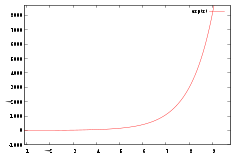
\includegraphics[scale=0.2]{exponential.png}}
  \item<+-> Chaotic
    $\Rightarrow$ small syntactic variations can lead
    to \alert{huge semantic variations}\\
    \visible<3->{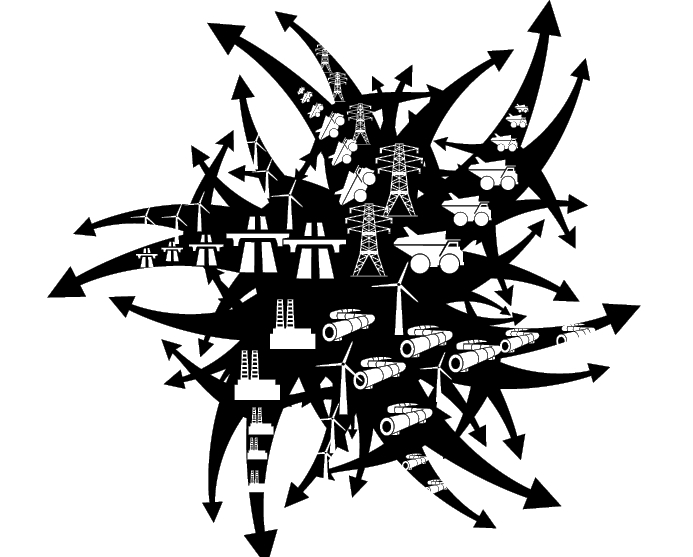
\includegraphics[scale=0.05]{chaos_theory.jpg}}
  \item<+-> Over-represented
    $\Rightarrow$ \alert{many programs with same semantics}\\
    \[x \AND y
    \equiv x \AND y \AND x
    \equiv \NOT(\NOT(x) \OR \NOT(y))
    \equiv \ldots\]
    
    \alert{less diversity} packed into the program space
  \end{itemize}
}

%\subsubsection{Over-representation}

\frame
{

  \frametitle{Over-representation}

  \begin{beamerboxesrounded}{Different syntax, same semantics}
    $
    \begin{array}{|c|c||c|c|c|c|c|c|}
      \hline
      x & y & x \AND y
      \only<2->{& \NOT(\NOT y \OR \NOT x)} \only<3->{& x \AND x \AND y}
      \only<4->{& x \AND y \AND (\NOT z \OR z)} \only<5->{& \ldots}\\
      \hline
      0 & 0 & 0 \only<2->{& 0} \only<3->{& 0}
      \only<4->{& 0} \only<5->{& \ldots}\\
      0 & 1 & 0 \only<2->{& 0} \only<3->{& 0}
      \only<4->{& 0} \only<5->{& \ldots}\\
      1 & 0 & 0 \only<2->{& 0} \only<3->{& 0}
      \only<4->{& 0} \only<5->{& \ldots}\\
      1 & 1 & 1 \only<2->{& 1} \only<3->{& 1}
      \only<4->{& 1} \only<5->{& \ldots}\\
      \hline
    \end{array}
    $
  \end{beamerboxesrounded}

}

%\subsubsection{Syntactic vs Semantic De-correlation}

\frame
{
  \frametitle{Syntactic vs Semantic De-correlation}
  \begin{columns}[c]
    \column{1.5in}

    $f_1 = \structure<3>{x \AND (y \OR z)}$

%     {\small
%       \begin{tabular}{cccc}
%         $f_1$ & $=$ & $\structure<3>{x \AND (y \OR z)}$ & $=$ 
%         \Tree [.$\AND$ $x$ [.$\OR$ $y$ $z$ ] ]
%       \end{tabular}
%     }

    \begin{table}
      {\small
      $
      \begin{array}{|c|c|c||c|}
        \hline
        x & y & z & f_1\\
        \hline
        \structure<5>{0} & \structure<5>{0} & \structure<5>{0} & \alert<5>{0}\\
        \structure<6>{0} & \structure<6>{0} & \structure<6>{1} & \alert<6>{0}\\
        \structure<7>{0} & \structure<7>{1} & \structure<7>{0} & \alert<7>{0}\\
        \structure<8>{0} & \structure<8>{1} & \structure<8>{1} & \alert<8>{0}\\
        \structure<9>{1} & \structure<9>{0} & \structure<9>{0} & \alert<9>{0}\\
        \structure<10>{1} & \structure<10>{0} & \structure<10>{1} & \alert<10>{1}\\
        \structure<11>{1} & \structure<11>{1} & \structure<11>{0} & \alert<11>{1}\\
        \structure<12>{1} & \structure<12>{1} & \structure<12>{1} & \alert<12>{1}\\
        \hline
      \end{array}
      $
      }
    \end{table}

    \column{1.5in}

    $f_2 = \structure<3>{\alert<3>{\NOT}(x \AND (y \OR z))}$
    \begin{table}
      {\small
      $
      \begin{array}{|c|c|c||c|}
        \hline
        x & y & z & f_2\\
        \hline
        \structure<5>{0} & \structure<5>{0} & \structure<5>{0} & \alert<5>{1}\\
        \structure<6>{0} & \structure<6>{0} & \structure<6>{1} & \alert<6>{1}\\
        \structure<7>{0} & \structure<7>{1} & \structure<7>{0} & \alert<7>{1}\\
        \structure<8>{0} & \structure<8>{1} & \structure<8>{1} & \alert<8>{1}\\
        \structure<9>{1} & \structure<9>{0} & \structure<9>{0} & \alert<9>{1}\\
        \structure<10>{1} & \structure<10>{0} & \structure<10>{1} & \alert<10>{0}\\
        \structure<11>{1} & \structure<11>{1} & \structure<11>{0} & \alert<11>{0}\\
        \structure<12>{1} & \structure<12>{1} & \structure<12>{1} & \alert<12>{0}\\
        \hline
      \end{array}
      $
      }
    \end{table}
    
  \end{columns}

  \pause

  \begin{itemize}
  \item<+-> Syntactic distance between $f_1$ and $f_2$:
    \visible<+->{\alert<3>{1}}
  \item<+-> Semantic distance between $f_1$ and $f_2$:
    $\alert{\only<+>{1}\only<+>{2}\only<+>{3}\only<+>{4}
      \only<+>{5}\only<+>{6}\only<+>{7}\only<+>{8}}$
  \end{itemize}
}

\frame{
  
  \frametitle{Syntactic vs Semantic De-correlation}
  \begin{columns}[c]
    \column{1.5in}

    $g_1 = \structure<3-8>{\alert<3>{false}}$

    \begin{table}
    {\small
      $
        \begin{array}{|c|c|c||c|}
          \hline
          x & y & z & g_1\\
          \hline
          0 & 0 & 0 & 0\\
          0 & 0 & 1 & 0\\
          0 & 1 & 0 & 0\\
          0 & 1 & 1 & 0\\
          1 & 0 & 0 & 0\\
          1 & 0 & 1 & 0\\
          1 & 1 & 0 & 0\\
          \structure<10>{1} & \structure<10>{1} & \structure<10>{1} & \alert<10>{0}\\
          \hline
        \end{array}
      $
    }
    \end{table}
    \column{1.5in}

    $g_2 = \structure<3-8>{\alert<4>{x} \alert<5>{\AND} \alert<6>{y}
      \alert<7>{\AND} \alert<8>{z}}$
    \begin{table}
    {\small
      $
      \begin{array}{|c|c|c||c|}
        \hline
        x & y & z & g_2\\
        \hline
        0 & 0 & 0 & 0\\
        0 & 0 & 1 & 0\\
        0 & 1 & 0 & 0\\
        0 & 1 & 1 & 0\\
        1 & 0 & 0 & 0\\
        1 & 0 & 1 & 0\\
        1 & 1 & 0 & 0\\
        \structure<10>{1} & \structure<10>{1} & \structure<10>{1} & \alert<10>{1}\\
        \hline
      \end{array}
      $
    }
    \end{table}
    
  \end{columns}

  \pause

  \begin{itemize}
  \item<+-> Syntactic distance:
    $\alert<3-8>{
      \only<+>{1}\only<+>{2}\only<+>{3}\only<+>{4}\only<+>{5}\only<+->{6}}$
  \item<+-> Semantic distance:
    $\alert{\only<+>{1}}$
  \end{itemize}
}

\frame{
  \frametitle{Syntactic vs Semantic De-correlation}
  \begin{figure}
    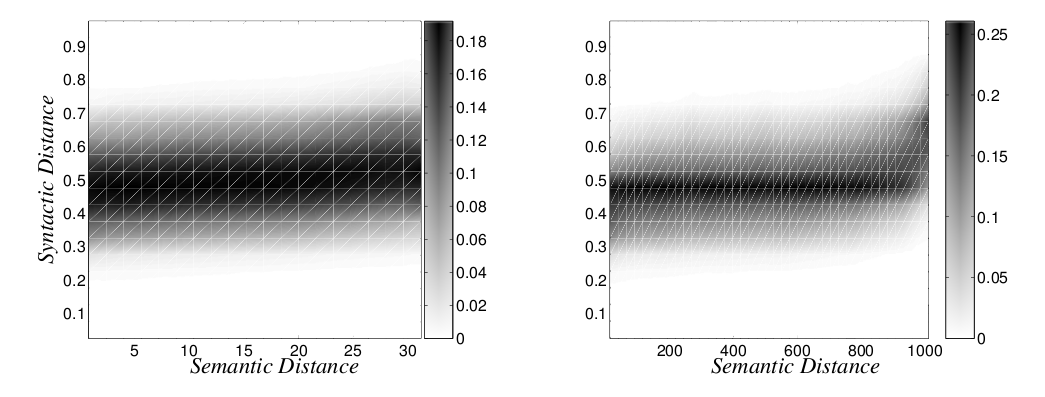
\includegraphics[scale=0.4]{synvssem.png}
    \caption{Syntactic vs semantic distance
      for random formulae with arities five (left) and ten
      (right). \emph{Extracted from Moshe Looks PhD thesis.}}
  \end{figure}
}

\subsection{What are Programs in Normal Forms?}

\frame
{

  \frametitle{Programs in Normal Forms}

  \begin{enumerate}
    \item unique representation (possibly the shortest)
      \[x \AND y
      \alert{\rlap{------------------------------------------------}}
      \equiv x \AND y \AND x
      \equiv \NOT(\NOT(x) \OR \NOT(y))
      \equiv \ldots  \]

    \item interesting properties
      $\Rightarrow$ program space more regular
      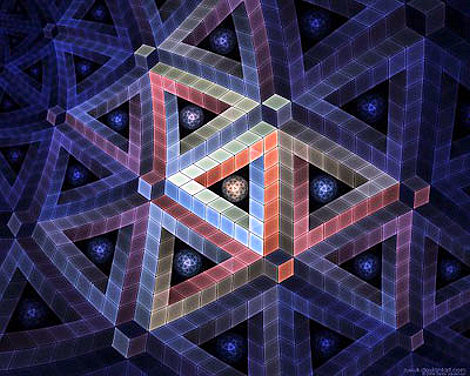
\includegraphics[scale=0.1]{impossible_space.jpg}
    \end{enumerate}
}

\subsection{Effects of Reducing Programs in Normal Forms}
% \frame
% {
%   \frametitle{Why Reducing Programs in Normal Forms?}

%   \begin{enumerate}
%   \item<1-> Avoid over-representation
%   \item<2-> Increase syntactic vs semantic correlation 
%   \item<3-> Improve hierarchical structure 
%   \item<4-> Smaller programs take less memory and usually run faster
%   \end{enumerate}
% }

%\subsubsection{Avoid over-representation}

\frame
{
  \frametitle{Avoiding over-representation}
  
  \only<1>{Before}\only<2>{After} reduction:\\

  \begin{columns}
    \column{1in}
    
    \only<1>{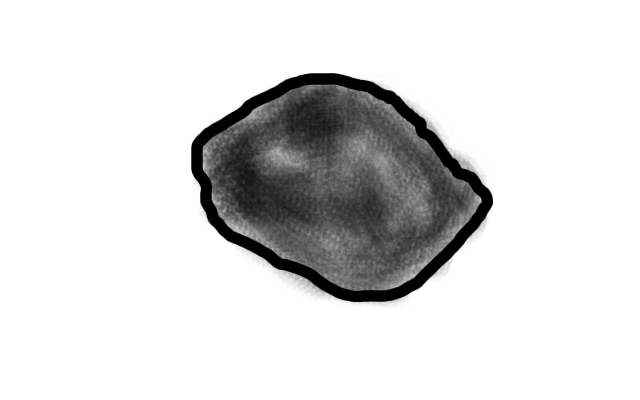
\includegraphics[scale=0.25]{program_space.png}}
    \only<2>{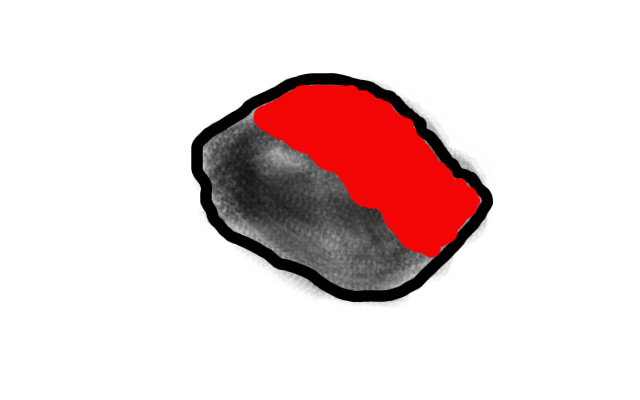
\includegraphics[scale=0.25]{program_space_reduct.png}}
    
    \column{1.5in}
    Program space
  \end{columns}

%    \caption{Program space \only<1>{before}\only<2>{after} reduction}
%  \end{figure}

  $x \AND y
  \visible<2>{\alert{\rlap{------------------------------------------------}}}
  \equiv x \AND y \AND x
  \equiv \NOT(\NOT(x) \OR \NOT(y))
  \equiv \ldots $\\
  
  $x \OR y
  \visible<2>{\alert{\rlap{------------------------------------------------}}}
  \equiv x \OR y \OR x
  \equiv \NOT(\NOT(x) \AND \NOT(y))
  \equiv \ldots $\\

  $x \AND y \AND z
  \visible<2>{\alert<2>{\rlap{---------------------------------------}}}
  \equiv x \AND y \AND z \AND x \AND y \AND z \equiv \ldots $\\
  
  $x \AND y \AND \NOT(z)
  \visible<2>{\alert{\rlap{------------------------------------------------}}}
  \equiv x \AND y \AND \NOT(z) \AND x \AND y \AND \NOT(z) \equiv \ldots $\\

  $\ldots$\\

  \pause
}

%\subsubsection{Increase Syntactic vs Semantic Correlation}

\frame
{
  \frametitle{Increase Syntactic vs Semantic Correlation}

  Before reduction

  \begin{columns}[c]
    \column{1.5in}

    $f_1 = x \AND (y \OR z)$

    \begin{table}
      {\small
      $
      \begin{array}{|c|c|c||c|}
        \hline
        x & y & z & f_1\\
        \hline
        0 & 0 & 0 & 0\\
        0 & 0 & 1 & 0\\
        0 & 1 & 0 & 0\\
        0 & 1 & 1 & 0\\
        1 & 0 & 0 & 0\\
        1 & 0 & 1 & 1\\
        1 & 1 & 0 & 1\\
        1 & 1 & 1 & 1\\
        \hline
      \end{array}
      $
      }
    \end{table}

    \column{1.5in}

    $f_2 =   \NOT (x \AND (y \OR z))$
    \begin{table}
      {\small
      $
      \begin{array}{|c|c|c||c|}
        \hline
        x & y & z & f_2\\
        \hline
        0 & 0 & 0 & 1\\
        0 & 0 & 1 & 1\\
        0 & 1 & 0 & 1\\
        0 & 1 & 1 & 1\\
        1 & 0 & 0 & 1\\
        1 & 0 & 1 & 0\\
        1 & 1 & 0 & 0\\
        1 & 1 & 1 & 0\\
        \hline
      \end{array}
      $
      }
    \end{table}
    
  \end{columns}

  \begin{itemize}
  \item Syntactic distance between $f_1$ and $f_2$: $1$
  \item Semantic distance between $f_1$ and $f_2$: $8$
  \end{itemize}
}


\frame
{
  \frametitle{Increase Syntactic vs Semantic Correlation}

  After reduction

  \begin{columns}[c]
    \column{1.5in}

    $f_1 = \structure<2-6>{x \alert<3>{\AND} (y \alert<5>{\OR} z)}$

    \begin{table}
      {\small
      $
      \begin{array}{|c|c|c||c|}
        \hline
        x & y & z & f_1\\
        \hline
        0 & 0 & 0 & 0\\
        0 & 0 & 1 & 0\\
        0 & 1 & 0 & 0\\
        0 & 1 & 1 & 0\\
        1 & 0 & 0 & 0\\
        1 & 0 & 1 & 1\\
        1 & 1 & 0 & 1\\
        1 & 1 & 1 & 1\\
        \hline
      \end{array}
      $
      }
    \end{table}

    \column{1.5in}

    $f_2 = \structure<2-6>{\alert<2>{\NOT} x \alert<3>{\OR} (\alert<4>{\NOT} y \alert<5>{\AND} \alert<6>{\NOT} z)}$
    \begin{table}
      {\small
      $
      \begin{array}{|c|c|c||c|}
        \hline
        x & y & z & f_2\\
        \hline
        0 & 0 & 0 & 1\\
        0 & 0 & 1 & 1\\
        0 & 1 & 0 & 1\\
        0 & 1 & 1 & 1\\
        1 & 0 & 0 & 1\\
        1 & 0 & 1 & 0\\
        1 & 1 & 0 & 0\\
        1 & 1 & 1 & 0\\
        \hline
      \end{array}
      $
      }
    \end{table}
    
  \end{columns}

  \begin{itemize}
  \item Syntactic distance between $f_1$ and $f_2$:
    \only<+>{?}
    \alert{\only<+>{1}\only<+>{2}\only<+>{3}\only<+>{4}\only<+>{5}}
  \item Semantic distance between $f_1$ and $f_2$: $8$
  \end{itemize}
}

\frame{
  
  \frametitle{Increase Syntactic vs Semantic Correlation}

  Before and after reduction\\

  \begin{columns}[c]
    \column{1.5in}

    $g_1 = false$

    \begin{table}
    {\small
      $
        \begin{array}{|c|c|c||c|}
          \hline
          x & y & z & g_1\\
          \hline
          0 & 0 & 0 & 0\\
          0 & 0 & 1 & 0\\
          0 & 1 & 0 & 0\\
          0 & 1 & 1 & 0\\
          1 & 0 & 0 & 0\\
          1 & 0 & 1 & 0\\
          1 & 1 & 0 & 0\\
          1 & 1 & 1 & 0\\
          \hline
        \end{array}
      $
    }
    \end{table}
    \column{1.5in}

    $g_2 = x \AND y \AND z$
    \begin{table}
    {\small
      $
      \begin{array}{|c|c|c||c|}
        \hline
        x & y & z & g_2\\
        \hline
        0 & 0 & 0 & 0\\
        0 & 0 & 1 & 0\\
        0 & 1 & 0 & 0\\
        0 & 1 & 1 & 0\\
        1 & 0 & 0 & 0\\
        1 & 0 & 1 & 0\\
        1 & 1 & 0 & 0\\
        1 & 1 & 1 & 1\\
        \hline
      \end{array}
      $
    }
    \end{table}
    
  \end{columns}

  \begin{itemize}
  \item Syntactic distance: 6
  \item Semantic distance: 1
  \end{itemize}
}

\frame{
  \frametitle{Increase Syntactic vs Semantic Correlation}

  Before reduction\\

  \begin{figure}
    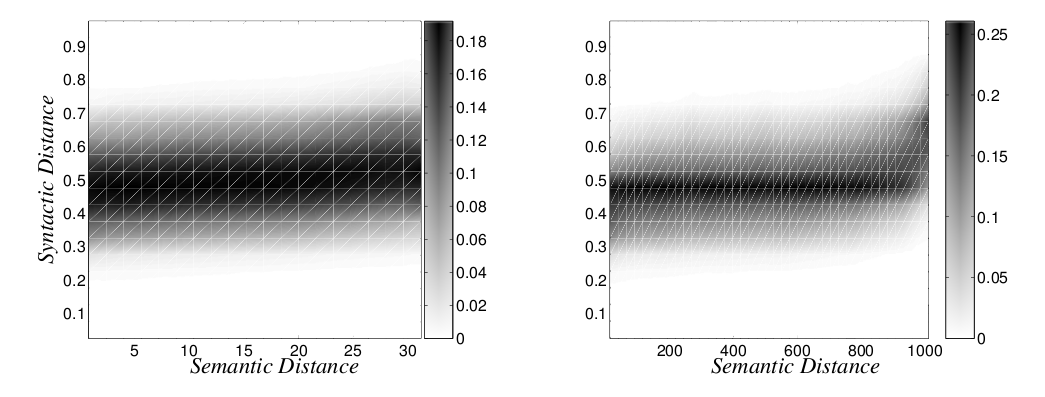
\includegraphics[scale=0.4]{synvssem.png}
    \caption{Syntactic vs semantic distance
      for random formulae with arities five (left) and ten
      (right). \emph{Extracted from Moshe Looks PhD thesis.}}
  \end{figure}
}

\frame{
  \frametitle{Increase Syntactic vs Semantic Correlation}

  After reduction\\

  \begin{figure}
    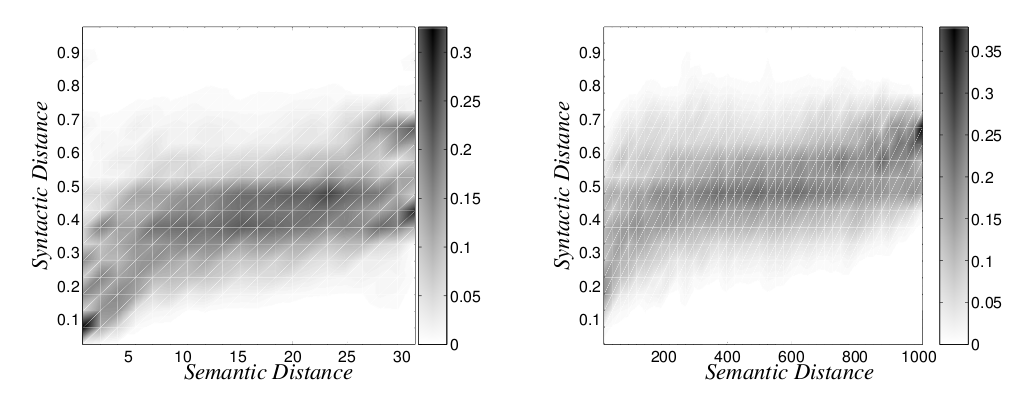
\includegraphics[scale=0.4]{synvssem_reduct.png}
    \caption{Syntactic vs semantic distance
      for random formulae in normal form with arities five (left) and ten
      (right). \emph{Extracted from Moshe Looks PhD thesis.}}
  \end{figure}
}

%\subsubsection{Improve Structure, interpretable, hierarchy}

\frame
{
  \frametitle{Improve Structure, interpretable, hierarchy}

  Before reduction: \visible<4>{$f_L$ and $f_R$ are not independent.}\\


  \begin{columns}
    
    \column{1.5in}

    $\NOT(x \OR y) \AND (\NOT(y) \OR z)$

    \column{0.2in}

    $=$

    \column{1in}

    \Tree [.$\AND$ [.{\color<2>{green} $\NOT$}
    [.{\color<2>{green}$\OR$}
    {\color<2>{green}$x$}
    {\color<2>{green}\structure<4>{$y$}} ] ]
    [.{\color<3>{red}$\OR$}
    [.{\color<3>{red}$\NOT$ \structure<4>{$y$}} ] {\color<3>{red}z} ] ]

    \column{0.2in}

    $=$

    \column{1in}

    \Tree [.$\AND$ {\color<2>{green}$f_L$} {\color<3>{red}$f_R$} ] 

  \end{columns}

}

\frame
{
  \frametitle{Improve Structure, interpretable, hierarchy}

  After reduction: $g_L$ and $g_R$ are \alert{independent}.\\
  \begin{columns}
    
    \column{1in}

    $\NOT x \AND \NOT y$

    \column{0.2in}

    $=$

    \column{1in}

    \Tree [.$\AND$ $\NOT x$ $\NOT y$ ]

    \column{0.2in}

    $=$

    \column{1in}

    \Tree [.$\AND$ $g_L$ $g_R$ ] 

  \end{columns}

  \pause

  \begin{beamerboxesrounded}{Benefice}
    \begin{itemize}
    \item Easier to understand
    \item Better hierarchical structure
    \end{itemize}
  \end{beamerboxesrounded}

}

\frame
{
  \frametitle{To sum up}
  
  Reduction allows us to:
  \begin{enumerate}
  \item Avoid \alert{over-representation}
  \item Increase \alert{syntactic vs semantic correlation}
  \item \alert{Improve structure}
  \item Smaller programs take \alert{less memory} and usually run faster
  \end{enumerate}


  \begin{beamerboxesrounded}{Conclusion}
    Reduction is good!
  \end{beamerboxesrounded}
}

\frame
{

  \frametitle{But beware!}
  
  Reduction to normal form is:
  \begin{itemize}
  \item<+-> undecidable for recursive functions
      \visible<1->{
\includegraphics[scale=0.08]{computer_undec3.jpg}}
    
  \item<+-> undecidable for primitive recursive functions
      \visible<2->{
\includegraphics[scale=0.08]{computer_undec3.jpg}}
  \item<+-> NP-hard for Boolean functions
      \visible<3->{
\includegraphics[scale=0.08]{computer_hard.jpg}}
  \end{itemize}
  \pause
  \begin{beamerboxesrounded}{In practice}
    \begin{itemize}
    \item<+-> \alert{incomplete} reduction methods
    \item<+-> rely on \alert{heuristics}
    \item<+-> trade-off between \alert{efficiency} and completeness 
    \end{itemize}
  \end{beamerboxesrounded}

}
\section{The Reduct Toolkit}

\frame
{
  \frametitle{The Reduct Toolkit}

  \begin{itemize}[<+->]
  \item Part of the OpenCog framework
  \item Coded in C++
  \item Handles the following domains
    \begin{itemize}
    \item Boolean
    \item Continuous
    \item numerico-boolean
    \item actions perceptions to control agent in virtual world
    \end{itemize}
  \end{itemize}
}

\subsection{Recall of Combo}

\frame
{

  \frametitle{Reduct Operates on Combo}

  Combo is:
  \begin{itemize}
  \item<+-> Programmatic language of MOSES
  \item<+-> Syntactic tree in prefix notation\\
    \begin{columns}
      
      \column{0.5in}
      \Tree [.$\AND$ \alert<+>{$x$} [.$\OR$ \alert<3>{$y$} $\NOT \alert<3>{z}$ ] ]
      
      \column{0.1in}
      $\Leftrightarrow$

      \column{2.4in}
      \tt{and(\alert<3>{\#1} or(\alert<3>{\#2} not(\alert<3>{\#3})))}
      
    \end{columns}
  \item<+-> Boolean: {\tt and}, {\tt or}, {\tt not}, {\tt true}, {\tt false}
  \item<+-> Continuous:
    {\tt +}, {\tt *}, {\tt /}, {\tt exp}, {\tt log}, {\tt sin}
  \item<+-> Numerico-Boolean:
    {\tt 0<}, {\tt impulse}, {\tt contin\_if}
  \item<+-> Action:
    {\tt and\_seq},
    %{\tt or\_seq}, {\tt exec\_seq},
    {\tt action\_if},
    {\tt action\_while},
    %{\tt repeat\_n}, 
    $\ldots$
  \item<+-> Higher order: {\it procedure\_name{\tt (}arity{\tt) := }body}
  \end{itemize}

}

\subsection{How it works}

\frame
{
  \frametitle{Reduction}

  \begin{beamerboxesrounded}{How it works}
    Apply series of reduction rules according to a given strategy.
  \end{beamerboxesrounded}

  \begin{center}
    {\tiny
      \begin{tikzpicture}[node distance   = 1.4 cm]
        \GraphInit[vstyle=Shade]
        \tikzset{LabelStyle/.style =   {draw,
            fill  = yellow,
            text  = red}}
        \Vertex[L=$\downarrow R_5$]{DR5}
        \EA[L=$\uparrow R_3$](DR5){UR3}
        \EA[L=$\uparrow R_4$](UR3){UR4}
        \EA[L=$\downarrow R_1$](UR4){DR1}
        \EA[L=$ENF$](DR1){ENF}
        \EA[L=$\downarrow R_9$](ENF){DR9}
        \EA[L=$\downarrow R_8$](DR9){DR8}
        \EA[L=$\downarrow R_2$](DR8){DR2}
        \tikzset{EdgeStyle/.append style = {->}}
        \Edge(DR5)(UR3)
        \Edge(UR3)(UR4)
        \Edge(UR4)(DR1)
        \Edge(DR1)(ENF)
        \Edge(ENF)(DR9)
        \Edge(DR9)(DR8)
        \Edge(DR8)(DR2)
        \tikzset{EdgeStyle/.append style = {->, bend left}}
        \Edge[label=Iterative](DR8)(UR4)
      \end{tikzpicture}
    }
  \end{center}
  

}

\frame
{
  \frametitle{Reduct Rules}

  Example of reduction rules in the Boolean domain:
  \begin{itemize}
  \item<+-> $R_4$: {\tt and($X$)} $\rightarrow$ $X$
  \item<+-> $R_5$: {\tt not(not($X$))} $\rightarrow$ $X$
  \item<+-> $R_8$: {\tt or($X$ true)} $\rightarrow$ {\tt true}
%  \item<+-> $\ldots$
  \end{itemize}
  \pause
  In the continuous domain:
  \begin{itemize}
  \item<+-> $R_{13}$: {\tt $X$/$Z$+$Y$/$Z$} $\rightarrow$ {\tt ($X$+$Y$)/$Z$}
  \item<+-> $R_{21}$: {\tt exp($X$)*exp($Y$)} $\rightarrow$ {\tt exp($X$+$Y$)}
%  \item<+-> $\ldots$
  \end{itemize}
  \pause
  In the action domain:
  \begin{itemize}
  \item<+-> $R_{43}$: {\tt action\_if($B$ $X$ $Y$)} $\rightarrow$
    $X$ $\ $ \structure{if $B$ is reducible to {\tt true}}
  \item<+-> $R_{51}$: {\tt action\_while($X$ $\ldots$ $X$)} $\rightarrow$
    {\tt action\_while($X$)}
%  \item<+-> $\ldots$
  \end{itemize}

  \pause

  \begin{center}
     \alert{about 85 rules in total...}
  \end{center}
}

\frame
{
  \frametitle{Combining the reduction rules}

  \begin{center}
    {\tiny
      \begin{tikzpicture}[node distance   = 1.4 cm]
        \GraphInit[vstyle=Shade]
        \tikzset{LabelStyle/.style =   {draw,
            fill  = yellow,
            text  = red}}
        \Vertex[L=$\downarrow R_5$]{DR5}
        \EA[L=$\uparrow R_3$](DR5){UR3}
        \EA[L=$\uparrow R_4$](UR3){UR4}
        \EA[L=$\downarrow R_1$](UR4){DR1}
        \EA[L=$ENF$](DR1){ENF}
        \EA[L=$\downarrow R_9$](ENF){DR9}
        \EA[L=$\downarrow R_8$](DR9){DR8}
        \EA[L=$\downarrow R_2$](DR8){DR2}
        \tikzset{EdgeStyle/.append style = {->}}
        \Edge(DR5)(UR3)
        \Edge(UR3)(UR4)
        \Edge(UR4)(DR1)
        \Edge(DR1)(ENF)
        \Edge(ENF)(DR9)
        \Edge(DR9)(DR8)
        \Edge(DR8)(DR2)
        \tikzset{EdgeStyle/.append style = {->, bend left}}
        \Edge[label=Iterative](DR8)(UR4)
      \end{tikzpicture}
    }
  \end{center}

  \pause

  \begin{columns}
    \column{1in}

    \only<1-9>{
    {\tiny
      \begin{tikzpicture}[node distance   = 1.4 cm]
        \GraphInit[vstyle=Shade]
        \tikzset{LabelStyle/.style =   {draw,
            fill  = yellow,
            text  = red}}
        \Vertex[L=$\downarrow R_i$]{DRi}
      \end{tikzpicture}
    }
    }

    \only<10-17>{
    {\tiny
      \begin{tikzpicture}[node distance   = 1.4 cm]
        \GraphInit[vstyle=Shade]
        \tikzset{LabelStyle/.style =   {draw,
            fill  = yellow,
            text  = red}}
        \Vertex[L=$\uparrow R_i$]{DRi}
      \end{tikzpicture}
    }
    }

    \column{1in}
    \Tree [.\alert<2,17>{$\AND$} [.\alert<3,13>{$\NOT$}
    [.\alert<4,12>{$\OR$} \alert<5,10>{$x$} \alert<6,11>{$y$} ] ]
    [.\alert<7,16>{$\OR$} 
    [.\alert<8,14>{$\NOT y$} ] \alert<9,15>{z} ] ]

    \column{1.5in}
    Apply $R_i$ from the \only<1-9>{root down to the leaves.}
    \only<10-17>{leaves up to the root.}
    
  \end{columns}

}

\frame
{
  \frametitle{Combining the reduction rules}

  \begin{center}
    {\tiny
      \begin{tikzpicture}[node distance   = 1.4 cm]
        \GraphInit[vstyle=Shade]
        \tikzset{LabelStyle/.style =   {draw,
            fill  = yellow,
            text  = red}}
        \Vertex[L=$\downarrow R_5$]{DR5}
        \EA[L=$\uparrow R_3$](DR5){UR3}
        \EA[L=$\uparrow R_4$](UR3){UR4}
        \EA[L=$\downarrow R_1$](UR4){DR1}
        \EA[L=$ENF$](DR1){ENF}
        \EA[L=$\downarrow R_9$](ENF){DR9}
        \EA[L=$\downarrow R_8$](DR9){DR8}
        \EA[L=$\downarrow R_2$](DR8){DR2}
        \tikzset{EdgeStyle/.append style = {->}}
        \Edge(DR5)(UR3)
        \Edge(UR3)(UR4)
        \Edge(UR4)(DR1)
        \Edge(DR1)(ENF)
        \Edge(ENF)(DR9)
        \Edge(DR9)(DR8)
        \Edge(DR8)(DR2)
        \tikzset{EdgeStyle/.append style = {->, bend left}}
        \Edge[label=Iterative](DR8)(UR4)
      \end{tikzpicture}
    }
  \end{center}

  %\pause

  \begin{columns}
    
    \column{1.5in}
    
    {\tiny
      \begin{tikzpicture}[node distance   = 4 cm]
        \GraphInit[vstyle=Shade]
        \tikzset{LabelStyle/.style =   {draw,
            fill  = yellow,
            text  = red}}
        \Vertex[L=$\ \ \ $]{DRa}
        \EA[L=$\ \ \ $](DRa){DRb}
        \tikzset{EdgeStyle/.append style = {->, bend left}}
        \Edge[label=Iterative](DRb)(DRa)
      \end{tikzpicture}
    }

    \column{1.5in}

    Repeat the strategy wrapped by {\tt Iterative}
    until the combo tree no longer changes.

  \end{columns}

}

\frame
{
  \frametitle{Combining the reduction rules}

  \begin{center}
    {\tiny
      \begin{tikzpicture}[node distance   = 1.4 cm]
        \GraphInit[vstyle=Shade]
        \tikzset{LabelStyle/.style =   {draw,
            fill  = yellow,
            text  = red}}
        \Vertex[L=$\downarrow R_5$]{DR5}
        \EA[L=$\uparrow R_3$](DR5){UR3}
        \EA[L=$\uparrow R_4$](UR3){UR4}
        \EA[L=$\downarrow R_1$](UR4){DR1}
        \EA[L=$ENF$](DR1){ENF}
        \EA[L=$\downarrow R_9$](ENF){DR9}
        \EA[L=$\downarrow R_8$](DR9){DR8}
        \EA[L=$\downarrow R_2$](DR8){DR2}
        \tikzset{EdgeStyle/.append style = {->}}
        \Edge(DR5)(UR3)
        \Edge(UR3)(UR4)
        \Edge(UR4)(DR1)
        \Edge(DR1)(ENF)
        \Edge(ENF)(DR9)
        \Edge(DR9)(DR8)
        \Edge(DR8)(DR2)
        \tikzset{EdgeStyle/.append style = {->, bend left}}
        \Edge[label=Iterative](DR8)(UR4)
      \end{tikzpicture}
    }
  \end{center}

  %\pause

  \begin{columns}
    
    \column{0.5in}
    
    {\tiny
      \begin{tikzpicture}[node distance   = 4 cm]
        \GraphInit[vstyle=Shade]
        \tikzset{LabelStyle/.style =   {draw,
            fill  = yellow,
            text  = red}}
        \Vertex[L=$ENF$]{ENF}
      \end{tikzpicture}
    }

    \column{2.5in}

    $ENF$: \alert{Elegant Normal Form} (Holman, '90).
    A strategy onto itself.\\
    \begin{itemize}
    \item<+-> Efficient
    \item<+-> Retain the structure (or even improve it) 
    \end{itemize}

  \end{columns}

}

\frame
{
  \frametitle{Combining the reduction rules}

  \begin{center}
    {\tiny
      \begin{tikzpicture}[node distance   = 1.4 cm]
        \GraphInit[vstyle=Shade]
        \tikzset{LabelStyle/.style =   {draw,
            fill  = yellow,
            text  = red}}
        \Vertex[L=$\downarrow R_5$]{DR5}
        \EA[L=$\uparrow R_3$](DR5){UR3}
        \EA[L=$\uparrow R_4$](UR3){UR4}
        \EA[L=$\downarrow R_1$](UR4){DR1}
        \EA[L=$ENF$](DR1){ENF}
        \EA[L=$\downarrow R_9$](ENF){DR9}
        \EA[L=$\downarrow R_8$](DR9){DR8}
        \EA[L=$\downarrow R_2$](DR8){DR2}
        \tikzset{EdgeStyle/.append style = {->}}
        \Edge(DR5)(UR3)
        \Edge(UR3)(UR4)
        \Edge(UR4)(DR1)
        \Edge(DR1)(ENF)
        \Edge(ENF)(DR9)
        \Edge(DR9)(DR8)
        \Edge(DR8)(DR2)
        \tikzset{EdgeStyle/.append style = {->, bend left}}
        \Edge[label=Iterative](DR8)(UR4)
      \end{tikzpicture}
    }
  \end{center}

  %\pause

  \begin{figure}
    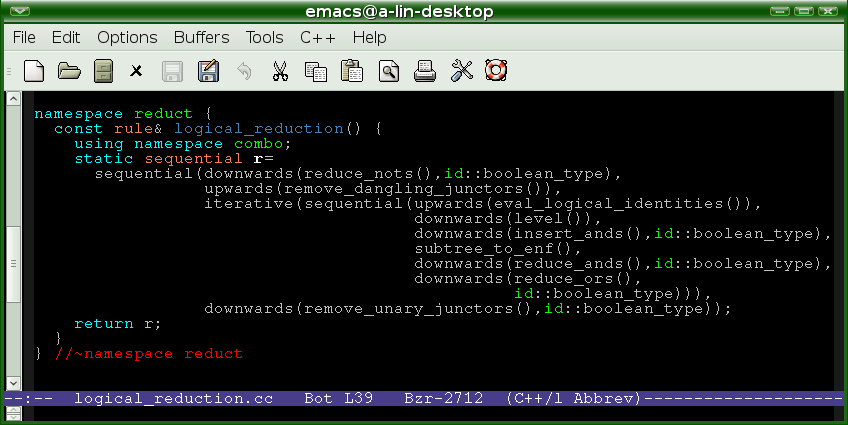
\includegraphics[scale=0.4]{logical_reduction.png}
    \caption{Snapshot of the code of the strategy of logical reduction}
  \end{figure}

}

\subsection{Demo...}

\subsection{What Remains to Be Implemented}

\frame
{
  \frametitle{What remains to be implemented}

  \begin{itemize}
  \item<+-> \structure{Boolean, continuous, action-perception}:
    virtually \alert{complete}
  \item<+-> \structure{Numerico-Boolean}:
    dealing with \alert{non-linear systems}
    like for instance {\tt 0<(*(+(\#1 1) +(\#1 1)))}
  \item<+-> \structure{Higher order, list, recursion}, etc:
    \alert{everything} remains to be done.
  \item<+-> Factorizing the rules, operator properties rather than
    operators themselves, for instance 
    \begin{itemize}
    \item {\tt +($X$ 0) $\rightarrow$ $X$}
    \item {\tt or($X$ false) $\rightarrow$ $X$}
    \end{itemize}
    2 instances of the {\it \structure{neutral\_element}} reduction rule.
  \end{itemize}
}


\end{document}
